%%%%%%%%%%%%%%%%%%%%%%%%%%%%%%%%%%%%%%%%%%%%%%%%%%%%%%%%%%%%%%%%%%%%%%%%%%%%%%%%
%Tutorial slides on Python.
%
% Author: FOSSEE
% Copyright (c) 2009, FOSSEE, IIT Bombay
%%%%%%%%%%%%%%%%%%%%%%%%%%%%%%%%%%%%%%%%%%%%%%%%%%%%%%%%%%%%%%%%%%%%%%%%%%%%%%%%

\documentclass[14pt,compress]{beamer}
%\documentclass[draft]{beamer}
%\documentclass[compress,handout]{beamer}
%\usepackage{pgfpages} 
%\pgfpagesuselayout{2 on 1}[a4paper,border shrink=5mm]

% Modified from: generic-ornate-15min-45min.de.tex
\mode<presentation>
{
  \usetheme{Warsaw}
  \useoutertheme{split}
  \setbeamercovered{transparent}
}

\usepackage[english]{babel}
\usepackage[latin1]{inputenc}
%\usepackage{times}
\usepackage[T1]{fontenc}

% Taken from Fernando's slides.
\usepackage{ae,aecompl}
\usepackage{mathpazo,courier,euler}
\usepackage[scaled=.95]{helvet}

\definecolor{darkgreen}{rgb}{0,0.5,0}

\usepackage{listings}
\lstset{language=Python,
    basicstyle=\ttfamily\bfseries,
    commentstyle=\color{red}\itshape,
  stringstyle=\color{darkgreen},
  showstringspaces=false,
  keywordstyle=\color{blue}\bfseries}

%%%%%%%%%%%%%%%%%%%%%%%%%%%%%%%%%%%%%%%%%%%%%%%%%%%%%%%%%%%%%%%%%%%%%%
% Macros
\setbeamercolor{emphbar}{bg=blue!20, fg=black}
\newcommand{\emphbar}[1]
{\begin{beamercolorbox}[rounded=true]{emphbar} 
      {#1}
 \end{beamercolorbox}
}
\newcounter{time}
\setcounter{time}{0}
\newcommand{\inctime}[1]{\addtocounter{time}{#1}{\tiny \thetime\ m}}

\newcommand{\typ}[1]{\lstinline{#1}}

\newcommand{\kwrd}[1]{ \texttt{\textbf{\color{blue}{#1}}}  }

%%% This is from Fernando's setup.
% \usepackage{color}
% \definecolor{orange}{cmyk}{0,0.4,0.8,0.2}
% % Use and configure listings package for nicely formatted code
% \usepackage{listings}
% \lstset{
%    language=Python,
%    basicstyle=\small\ttfamily,
%    commentstyle=\ttfamily\color{blue},
%    stringstyle=\ttfamily\color{orange},
%    showstringspaces=false,
%    breaklines=true,
%    postbreak = \space\dots
% }


%%%%%%%%%%%%%%%%%%%%%%%%%%%%%%%%%%%%%%%%%%%%%%%%%%%%%%%%%%%%%%%%%%%%%%
% Title page
\title[Plotting using Python]{Plotting experimental data\\}

\author[FOSSEE] {FOSSEE}

\institute[IIT Bombay] {Department of Aerospace Engineering\\IIT Bombay}
\date[] {31, October 2009\\Day 1, Session 2}
%%%%%%%%%%%%%%%%%%%%%%%%%%%%%%%%%%%%%%%%%%%%%%%%%%%%%%%%%%%%%%%%%%%%%%

%\pgfdeclareimage[height=0.75cm]{iitmlogo}{iitmlogo}
%\logo{\pgfuseimage{iitmlogo}}


%% Delete this, if you do not want the table of contents to pop up at
%% the beginning of each subsection:
\AtBeginSubsection[]
{
  \begin{frame}<beamer>
    \frametitle{Outline}
    \tableofcontents[currentsection,currentsubsection]
  \end{frame}
}

\AtBeginSection[]
{
  \begin{frame}<beamer>
    \frametitle{Outline}
    \tableofcontents[currentsection,currentsubsection]
  \end{frame}
}

% If you wish to uncover everything in a step-wise fashion, uncomment
% the following command: 
%\beamerdefaultoverlayspecification{<+->}

%\includeonlyframes{current,current1,current2,current3,current4,current5,current6}

%%%%%%%%%%%%%%%%%%%%%%%%%%%%%%%%%%%%%%%%%%%%%%%%%%%%%%%%%%%%%%%%%%%%%%
% DOCUMENT STARTS
\begin{document}

\begin{frame}
  \titlepage
\end{frame}

\begin{frame}
  \frametitle{Outline}
  \tableofcontents
  % You might wish to add the option [pausesections]
\end{frame}

\section{Creating and running scripts}
\begin{frame}[fragile]
\frametitle{Python Scripts}
\begin{itemize}
\item Let us now put all the commands used in the review problem into a file. 
\item The following commands of IPython help us do this. 
\end{itemize}
\begin{lstlisting}
  In []: %hist
  In []: %hist -n
\end{lstlisting}
\end{frame}

\begin{frame}
\frametitle{Python Scripts\ldots}
  \begin{itemize}
    \item Open a new file in an \alert{editor}
    \item Copy and paste required lines from the output of \typ{\%hist -n}
    \item Save the file as \typ{first_plot.py}
  \end{itemize}
  \begin{itemize}
  \item run the file in IPython using \typ{\%run first_plot.py}\\
  \end{itemize}
\end{frame}

\section{Plotting Points}
\begin{frame}[fragile]
\frametitle{Simple Pendulum - L and T}
  \begin{itemize}
    \item Given data of Length and Time-period of a Simple pendulum 
    \item $T^2 = \frac{4\pi^2}{g}L$\\ \alert{{$L$} and {$T^2$} vary linearly}
    \item We wish to plot L vs. \alert{$T^2$}
  \end{itemize}    
\begin{lstlisting}
In []: L = [0.1,  0.2,  0.3,  
            0.4,  0.5,  0.6,  
            0.7,  0.8,  0.9]
In []: T = [0.6529, 0.8485, 1.0590, 
            1.2390, 1.4124, 1.5061, 
            1.6441, 1.7949, 1.8758]
\end{lstlisting}
\end{frame}

\begin{frame}[fragile]
\frametitle{Plotting $L$ vs. $T^2$}
\begin{itemize}
\item We must square each of the values in T
\item How to do it?
\item T is a \kwrd{list} and we use a \kwrd{for} loop to iterate over it
\end{itemize}
\end{frame}

\begin{frame}[fragile]
\frametitle{Plotting $L$ vs $T^2$}
\begin{lstlisting}
In []: TSq = []

In []: for t in T:
 ....:     TSq.append(t*t)

In []: plot(L, TSq)
Out[]: [<matplotlib.lines.Line2D object at 0xa5b05ac>]
\end{lstlisting}
\end{frame}

\begin{frame}[fragile]
\frametitle{Plotting points}
\begin{itemize}
\item But we want to plot points!
\end{itemize}
\begin{lstlisting}
  In []: clf()

  In []: plot(L, TSq, 'o')
  Out[]: [<matplotlib.lines.Line2D object at 0xac17e0c>]

  In []: clf()
  In []: plot(L, TSq, '.')
  Out[]: [<matplotlib.lines.Line2D object at 0xac17e0c>]
\end{lstlisting}
\end{frame}

\begin{frame}[fragile]
\frametitle{Additional Plotting Attributes}
\begin{itemize}
  \item \kwrd{'o'} - Dots
  \item \kwrd{'.'} - Smaller Dots
  \item \kwrd{'-'} - Lines
  \item \kwrd{'- -'} - Dashed lines
\end{itemize}
\end{frame}

\begin{frame}{New Concepts}
  \begin{itemize}
    \item lists
    \item \typ{for}
  \end{itemize}
\end{frame}

\section{Lists}
\begin{frame}[fragile]
  \frametitle{How to create and use lists?}
\begin{lstlisting}
In []: mtlist = [] #Empty List

In []: lst = [1,2,3,4] 

In []: lst[0]+lst[1]+lst[-1]
Out[]: 7
\end{lstlisting}
\end{frame}

\begin{frame}[fragile]
  \frametitle{List: Slicing}
list[initial:final:step]
\begin{lstlisting}
In []: lst[1:3]  # A slice.
Out[]: [2, 3]

In []: lst[1:-1]
Out[]: [2, 3]
\end{lstlisting}
\end{frame}

\begin{frame}[fragile]
  \frametitle{List methods}
\begin{lstlisting}
In []: lst.append(6)
In []: lst
Out[]: [1, 2, 3, 4, 5, 6]
\end{lstlisting}
%\inctime{10}
\end{frame}

\begin{frame}[fragile]
\frametitle{\texttt{for}}
Used to iterate over lists\\ Let us look at another example.
\begin{lstlisting}
In []: lst = [1,2,3,4,5,6]
In []: for num in lst:
 ....:     print num, num*num
 ....:    
1 1
2 4
3 9
4 16
5 25
6 36
\end{lstlisting}
\end{frame}

\begin{frame}[fragile]
\frametitle{Reading pendulum.txt}
\begin{itemize}
  \item We now wish to repeat the plot using the values from a file
  \item Given a file containing L vs. T values 
  \item Column1 - L; Column2 - T  
  \item Read the file
  \item Plot points for L vs. $T^2$ 
\end{itemize}
\end{frame}

\begin{frame}[fragile]
\frametitle{Reading pendulum.txt}
\begin{lstlisting}
In []: L = []
In []: T = []
In []: for line in open('pendulum.txt'):
  ....     points = line.split()
  ....     L.append(float(points[0]))
  ....     T.append(float(points[1]))
\end{lstlisting}
\begin{itemize}
\item We now have two lists L and T
\item Now, Repeat previous steps for plotting
\end{itemize}
\end{frame}

\begin{frame}[fragile]
\frametitle{Plotting from pendulum.txt}
\begin{lstlisting}
In []: TSq = []

In []: for t in T:
 ....:     TSq.append(t*t)

In []: plot(L, TSq, '.')
\end{lstlisting}
\end{frame}

\begin{frame}{New Concepts}
  \begin{itemize}
    \item File handling
    \item Strings
    \item Data-type conversion
  \end{itemize}
\end{frame}

\begin{frame}[fragile]
  \frametitle{Reading files \ldots}
\typ{In []: for line in open('pendulum.txt'):}
\begin{itemize}
\item opening file `pendulum.txt'
\item iterating through file using variable \typ{line}
\item \typ{line} is a \kwrd{string} variable
\end{itemize}
\end{frame}

\begin{frame}[fragile]
\frametitle{Strings}
Anything within ``quotes'' is a string!
\begin{lstlisting}
' This is a string '  
" This too! "
""" This one too! """
''' And one more! '''
\end{lstlisting}
\end{frame}

\begin{frame}[fragile]
\frametitle{Strings and \typ{split()}}
  \begin{lstlisting}
In []: line = 'hello world'

In []: a.split()
Out[]: ['hello', 'world']
  \end{lstlisting}
This is what happens with \typ{line}
  \begin{lstlisting}
In []: line = '1.2000e-01 7.4252e-01'

In []: line.split()
Out[]: ['1.2000e-01', '7.4252e-01']
  \end{lstlisting}
\end{frame}

\begin{frame}[fragile]
\frametitle{Getting floats from strings}
  \begin{lstlisting}
In []: type(points[0])
Out[]: <type 'str'>
  \end{lstlisting}
But, we need floating point numbers
  \begin{lstlisting}
In []: t = float(point[0])

In []: type(t)
Out[]: <type 'float'>
  \end{lstlisting}
\end{frame}

\begin{frame}[fragile]
\begin{figure}
%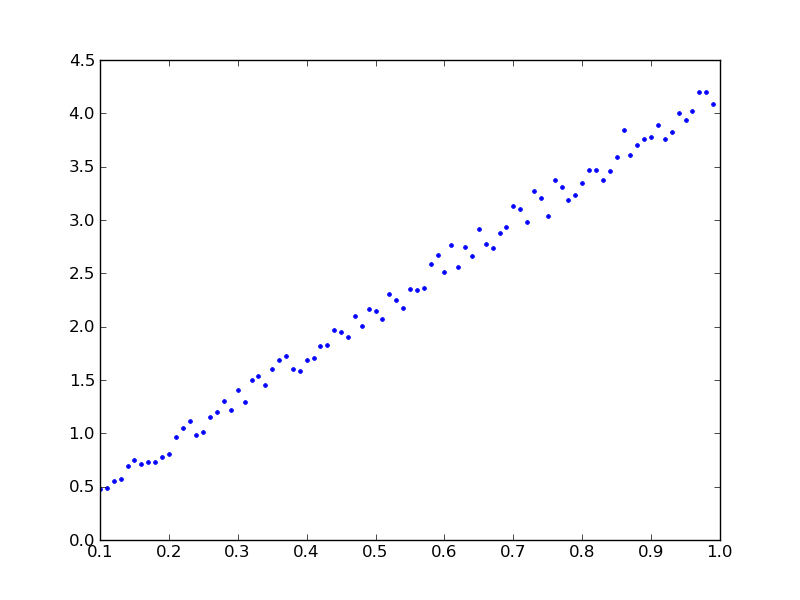
\includegraphics[width=3.5in]{data/L-Tsq.png}
\end{figure}
\vspace{-0.2in}
Coming up - \alert{Least Square Fit \ldots}
\end{frame}

\end{document}
